\documentclass{article}
\usepackage[margin=1in]{geometry}
\usepackage{parskip}
\usepackage{amsmath}
\usepackage{tikz}

\title{ISE 555 HW 3}
\author{Luke Pepin}
\date{October 5 2026}

\begin{document}
\maketitle

\section*{Question 1}
Substitute, flip to minimize, and drop the constant.

Minimize: $z' = -3x_1' + 5x_2' + 4x_3$

Subject to:
\begin{itemize}
    \item $7x_1' + 2x_2' - 3x_3 - e_1 = 11$
    \item $2x_1' + 4x_2' - 8x_3 = 29$
    \item $5x_1' + 3x_2' - 2x_3 + s_3 = 25$
    \item $x_1', x_2', x_3, e_1, s_3 \ge 0$
\end{itemize}

where $x_1 = x_1' + 1$, $x_2 = 7 - x_2'$, $z = 38 - z'$

\textbf{Substitution}

$7x_1' + 7 - 14 + 2x_2' - 3x_3 - e_1 = 4$

$-2x_1' - 2 + 28 - 4x_2' + 8x_3 = -3$, multiply by $-1$

$5x_1' + 5 - 21 + 3x_2' - 2x_3 + s_3 = 9$

\section*{Question 2}
Substitute and drop the constant.

Minimize: $z' = x_1' - 5x_2' + 5x_2'' - 7x_3' + 7x_3''$

Subject to:
\begin{itemize}
    \item $5x_1' - 2x_2' + 2x_2'' + 6x_3' - 6x_3'' - e_1 = 15$
    \item $3x_1' + 4x_2' - 4x_2'' - 9x_3' + 9x_3'' = 9$
    \item $7x_1' + 3x_2' - 3x_2'' + 5x_3' - 5x_3'' + s_3 = 23$
    \item $x_1', x_2', x_2'', x_3', x_3'', e_1, s_3 \ge 0$
\end{itemize}

where $x_1 = x_1' - 2$, $x_2 = x_2' - x_2''$, $x_3 = x_3' - x_3''$, $z = z' - 2$

\textbf{Substitution}

$5x_1' - 10 - 2x_2' + 2x_2'' + 6x_3' - 6x_3'' - e_1 = 5$

$3x_1' - 6 + 4x_2' - 4x_2'' - 9x_3' + 9x_3'' = 3$

$7x_1' - 14 + 3x_2' - 3x_2'' + 5x_3' - 5x_3'' + s_3 = 9$

\section*{Question 3}
Substitute, flip to minimize, and drop the constant.

Minimize: $z' = 6x_1' - 3x_2'$

Subject to:
\begin{itemize}
    \item $2x_1' + 5x_2' + e_1 = 95$
    \item $3x_1' + 2x_2' - s_2 = 35$
    \item $x_1', x_2', e_1, s_2 \ge 0$
\end{itemize}

where $x_1 = 15 - x_1'$, $x_2 = 15 - x_2'$, $z = 45 - z'$

\textbf{Substitution}

$30 - 2x_1' + 75 - 5x_2' - e_1 = 10$, multiply by $-1$

$45 - 3x_1' + 30 - 2x_2' + s_2 = 40$, multiply by $-1$

\section*{Question 4}
Add slack variables.

$x_1 + x_2 + s_1 = 5$

$x_1 + 2x_2 + s_2 = 6$

$x_1, x_2, s_1, s_2 \ge 0$

$m = 2$, $n = 4$, so $\binom{4}{2} = 6$ basic solutions. Set 2 variables to 0 and solve for the other 2.

\textbf{Basic Solutions}
\begin{itemize}
    \item $x_1 = x_2 = 0$: $s_1 = 5$, $s_2 = 6$, $(0,0)$ feasible
    \item $x_1 = s_1 = 0$: $x_2 = 5$, $s_2 = -4$, $(0,5)$ infeasible since $s_2 < 0$
    \item $x_1 = s_2 = 0$: $x_2 = 3$, $s_1 = 2$, $(0,3)$ feasible
    \item $x_2 = s_1 = 0$: $x_1 = 5$, $s_2 = 1$, $(5,0)$ feasible
    \item $x_2 = s_2 = 0$: $x_1 = 6$, $s_1 = -1$, $(6,0)$ infeasible since $s_1 < 0$
    \item $s_1 = s_2 = 0$: $(x_1 + 2x_2) - (x_1 + x_2) = 6 - 5$ so $x_2 = 1$ and $x_1 = 4$, $(4,1)$ feasible
\end{itemize}

\begin{minipage}{\linewidth}
\textbf{Sketch}

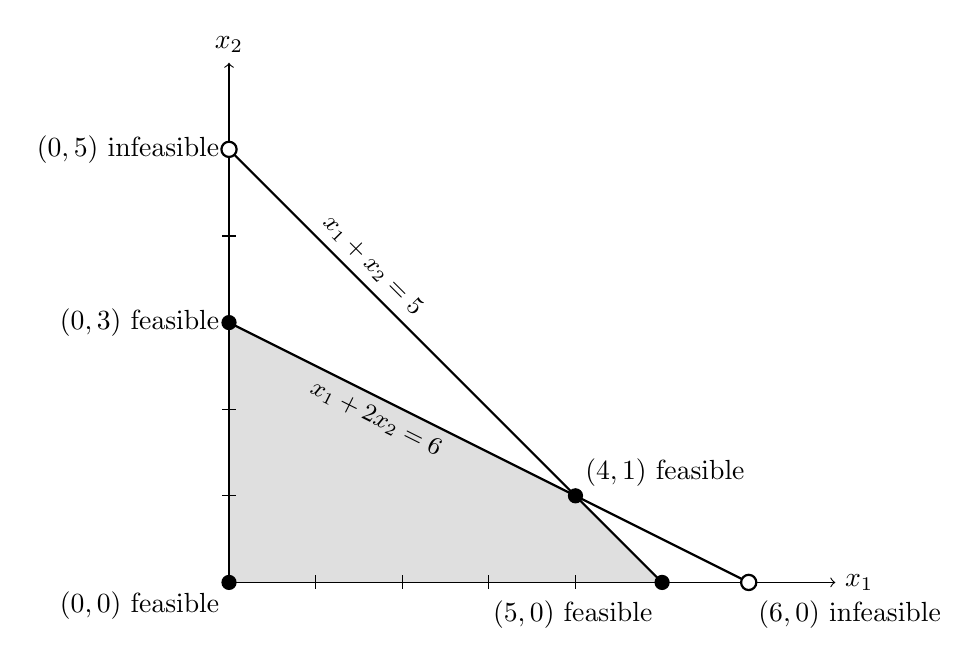
\begin{tikzpicture}[scale=1.1]
    \fill[gray!25] (0,0) -- (5,0) -- (4,1) -- (0,3) -- cycle;
    \draw[->] (0,0) -- (7,0) node[right] {$x_1$};
    \draw[->] (0,0) -- (0,6) node[above] {$x_2$};
    \foreach \x in {1,...,6} \draw (\x,0.08) -- (\x,-0.08);
    \foreach \y in {1,...,5} \draw (0.08,\y) -- (-0.08,\y);
    \draw[thick] (0,5) -- node[pos=0.3, sloped, above] {\small $x_1 + x_2 = 5$} (5,0);
    \draw[thick] (0,3) -- node[pos=0.3, sloped, below] {\small $x_1 + 2x_2 = 6$} (6,0);
    \foreach \p in {(0,0),(0,3),(5,0),(4,1)} \fill \p circle (2.5pt);
    \foreach \p in {(0,5),(6,0)} \draw[thick,fill=white] \p circle (2.5pt);
    \node[below left] at (0,0) {$(0,0)$ feasible};
    \node[left] at (0,3) {$(0,3)$ feasible};
    \node[left] at (0,5) {$(0,5)$ infeasible};
    \node[below left] at (5,-0.1) {$(5,0)$ feasible};
    \node[below right] at (6,-0.1) {$(6,0)$ infeasible};
    \node[above right] at (4,1) {$(4,1)$ feasible};
\end{tikzpicture}
\end{minipage}

The 4 feasible basic solutions are the 4 corners of the solution space.

\section*{Question 5}
Optimization can be used to help choose which location to close. Corporate has already shown a want and need to improve the company through the closure of a factory, and that decision was likely done through analysis of finance, engineering and business. Optimization attempts to do the same, just at a higher level of analysis, by developing a scientific model of the system. The issue of the locations is a maximization problem: how do we maximize the profit (throughput $-$ expenses) of the remaining locations? Given the closing of 1 of 3 factories, there are 3 combinations of factories which could survive. For each combination, through variables and figures for the expenses, profits, factory throughput, capacity, and demand for each of the five products, I would run an optimization to find the best production plan and the total company profit it gives. Then we can compare the 3 results and find the best combination. This is critical because the least efficient factory overall is not always the one to close. The remaining factories have to take on its work within their own capacity, and a factory that looks inefficient overall may be the best at making one product. Factors such as moving material into each other factory or the cost of closing may also be considered. The model can also be built to best improve whichever factor we account for, being cost, quality, Overall Equipment Effectiveness (OEE) or any other variable, while we set minimum and maximum values for each other.

\end{document}
